\documentclass{article}

\usepackage[heading=true]{ctex}
\usepackage[backref]{hyperref}
\usepackage{filecontents}
\usepackage{float}
\usepackage{graphicx}
\usepackage{geometry}
\usepackage{dirtree}
\usepackage{listings}
\usepackage{xcolor}
\usepackage{qtree}


\ctexset{
    section={
        number=\chinese{section},
        format+=\raggedright
    }
}
\geometry{a4paper, scale=0.7}


\title{实验五:GAN}
\author{1190200703 管健男}
\date{}


\begin{document}
\maketitle

\section{生成式对抗网络实现}

\subsection{GAN}

GAN主要包括两个部分:生成器和判别器。
对于实验中的任务,生成器负责生成一组点集,来拟合实验给定的点。
判别器负责判断当前生成的点是否在实验给定的点中。
每一次循环中,二者不断“对抗”,直到判别器无法区分生成器生成的假数据和原有数据。

GAN的loss函数为公式

\begin{equation}
    E_{x\sim p(x)}[\log D(x)] + E_{z\sim p(z)}[\log (1-D(G(z)))]
\end{equation}

其中D为判别器,G为生成器,而z为一个初始的随机噪音作为G的输入。
在pytorch中使用nn.BCELoss进行衡量此loss。

对于实验数据的拟合过程,如图所示

\begin{figure}[H]
    \begin{minipage}[H]{0.5\linewidth}
        \centering
        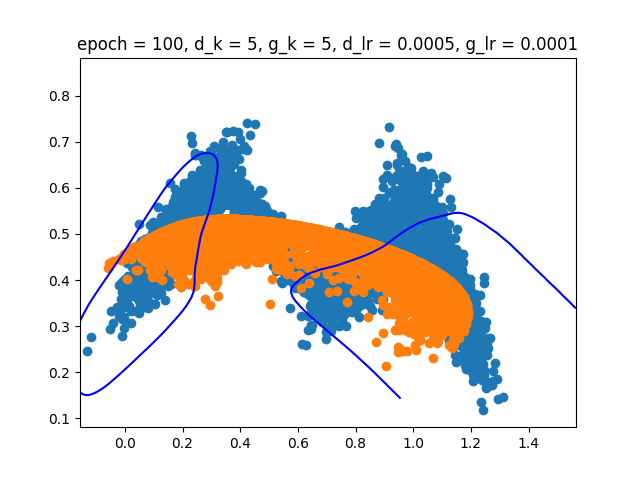
\includegraphics[width=\textwidth]{figures/GAN_0100.png}
    \end{minipage}
    \begin{minipage}[H]{0.5\linewidth}
        \centering
        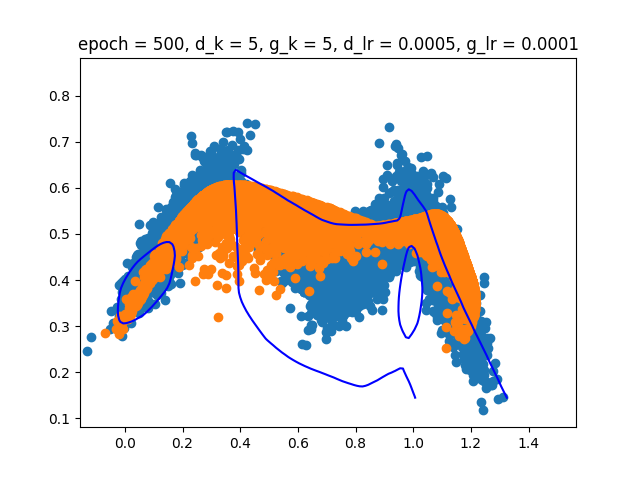
\includegraphics[width=\textwidth]{figures/GAN_0500.png}
    \end{minipage}
    \caption{GAN训练过程:第100和500个Epoch}
\end{figure}

\begin{figure}[H]
    \begin{minipage}[H]{0.5\linewidth}
        \centering
        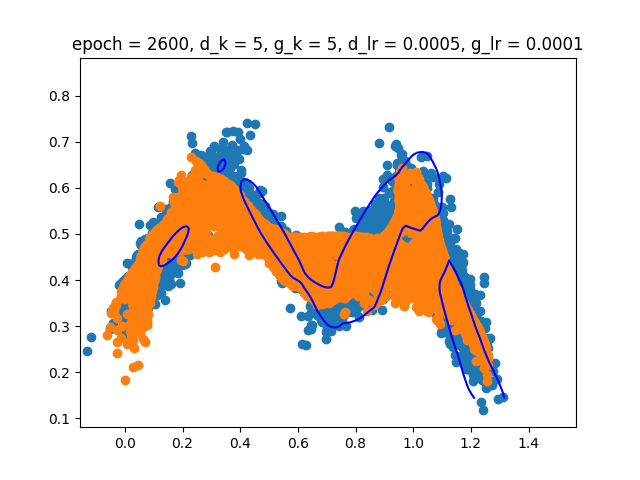
\includegraphics[width=\textwidth]{figures/GAN_2600.png}
    \end{minipage}
    \begin{minipage}[H]{0.5\linewidth}
        \centering
        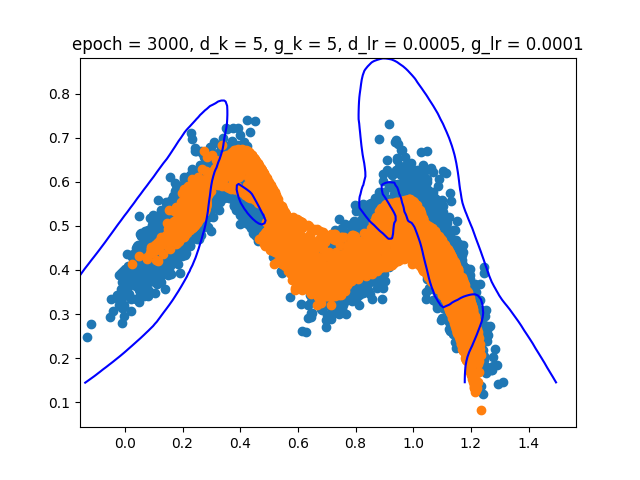
\includegraphics[width=\textwidth]{figures/GAN_3000.png}
    \end{minipage}
    \caption{GAN训练过程:第2600和3000个Epoch}
\end{figure}

其中D的学习率设置为$5 \times 10^{-4}$,G的学习率设置为$1 \times 10^{-4}$

可以看到,在这种情况下,GAN的收敛速度较快,但是并不稳定。
在epoch=3000时的拟合效果已经弱于2600时的效果。

\subsection{WGAN}

WGAN相比原始GAN的算法实现流程改进了四点:
\begin{enumerate}
    \item 判别器最后一层去掉sigmoid
    \item 生成器和判别器的loss不取log
    \item 每次更新判别器的参数之后把它们的绝对值截断到不超过一个固定常数c
    \item 不要用基于动量的优化算法(包括momentum和Adam),推荐RMSProp或SGD
\end{enumerate}

基于上述改进,WGAN的拟合过程如图

\begin{figure}[H]
    \begin{minipage}[H]{0.5\linewidth}
        \centering
        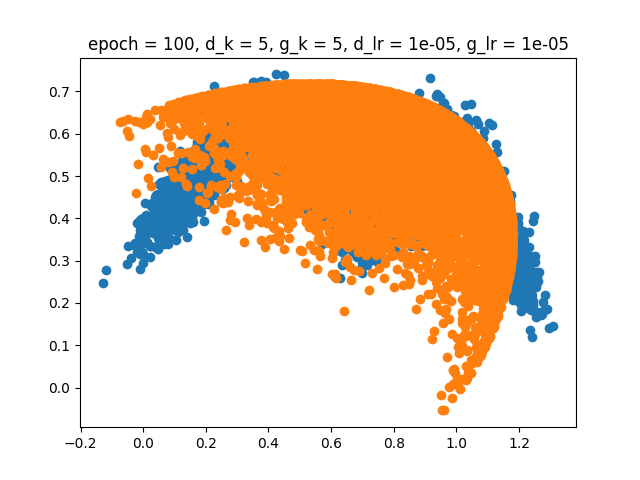
\includegraphics[width=\textwidth]{figures/WGAN_0100.png}
    \end{minipage}
    \begin{minipage}[H]{0.5\linewidth}
        \centering
        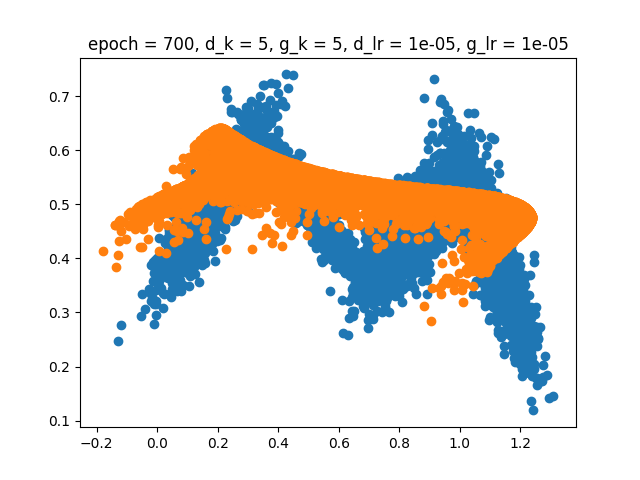
\includegraphics[width=\textwidth]{figures/WGAN_0700.png}
    \end{minipage}
    \caption{GAN训练过程:第100和700个Epoch}
\end{figure}

\begin{figure}[H]
    \begin{minipage}[H]{0.5\linewidth}
        \centering
        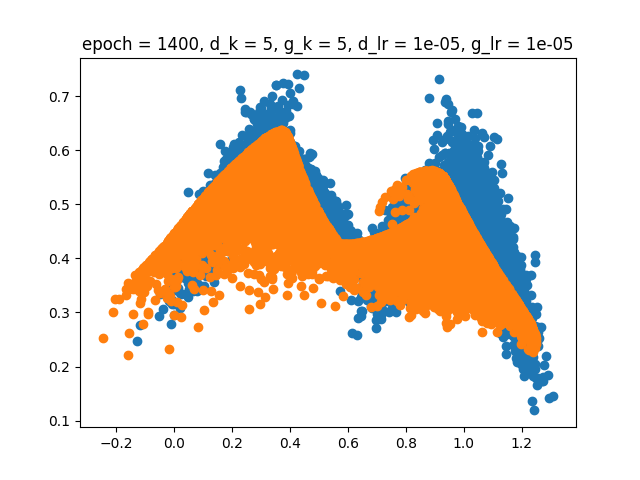
\includegraphics[width=\textwidth]{figures/WGAN_1400.png}
    \end{minipage}
    \begin{minipage}[H]{0.5\linewidth}
        \centering
        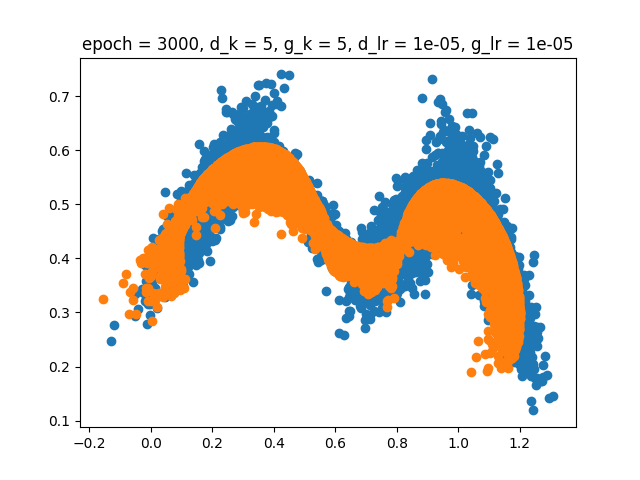
\includegraphics[width=\textwidth]{figures/WGAN_3000.png}
    \end{minipage}
    \caption{GAN训练过程:第1400和3000个Epoch}
\end{figure}

\subsection{WGAN-GP}

WGAN-GP用在loss上的梯度惩罚代替WGAN的判别器参数截取,拟合过程如图

\begin{figure}[H]
    \begin{minipage}[H]{0.5\linewidth}
        \centering
        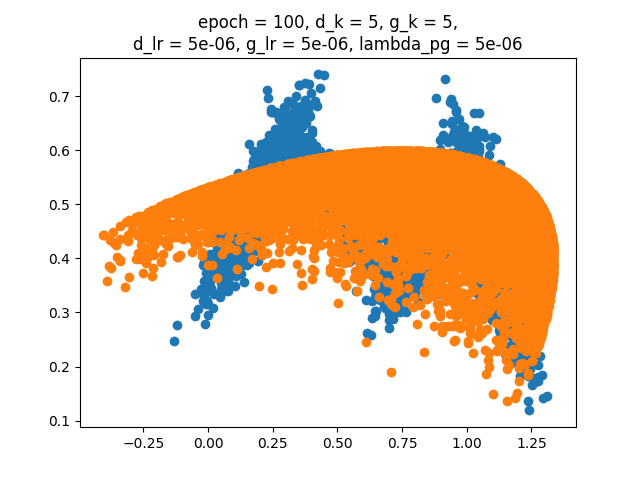
\includegraphics[width=\textwidth]{figures/WGANGP_0100.png}
    \end{minipage}
    \begin{minipage}[H]{0.5\linewidth}
        \centering
        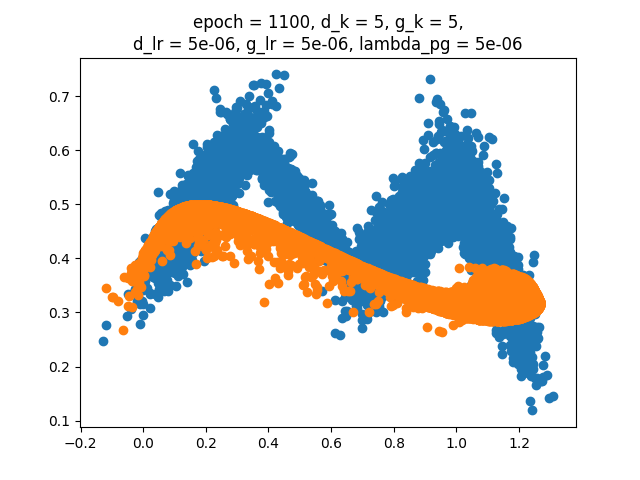
\includegraphics[width=\textwidth]{figures/WGANGP_1100.png}
    \end{minipage}
    \caption{GAN训练过程:第100和1100个Epoch}
\end{figure}

\begin{figure}[H]
    \begin{minipage}[H]{0.5\linewidth}
        \centering
        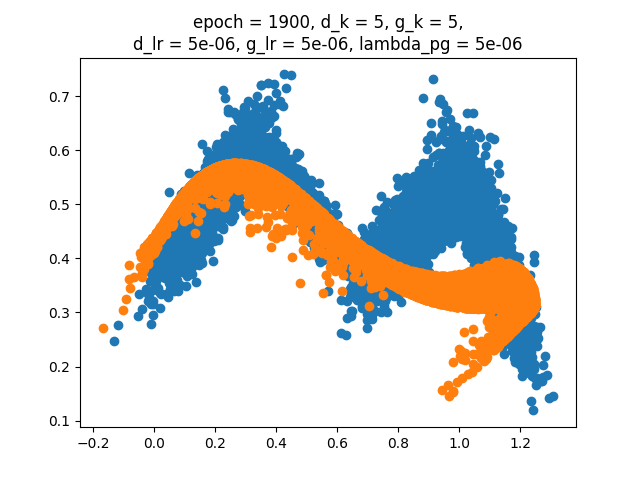
\includegraphics[width=\textwidth]{figures/WGANGP_1900.png}
    \end{minipage}
    \begin{minipage}[H]{0.5\linewidth}
        \centering
        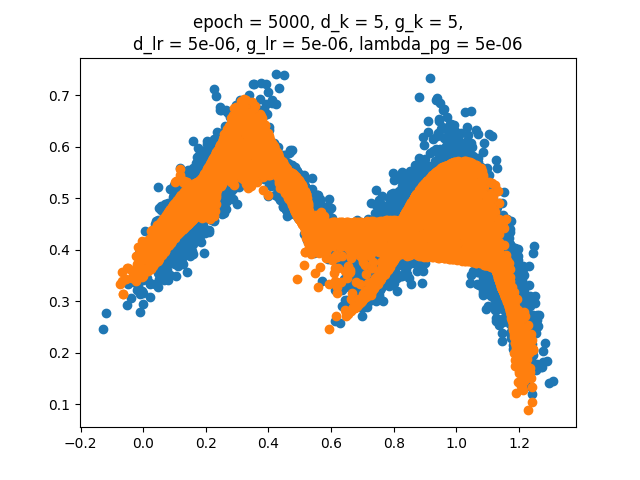
\includegraphics[width=\textwidth]{figures/WGANGP_5000.png}
    \end{minipage}
    \caption{GAN训练过程:第1900和5000个Epoch}
\end{figure}

\subsection{模型对比}

在实验中发现,WGAN和WGAN-GP的模型稳定性更高,拟合程度更好,
但是拟合速度较慢,可能需要更多次循环。

WGAN使用了RMSProp作为优化器,因为WGAN认为判别器越好,生成器梯度消失越严重。
因此并没有采用Adam优化器。
WGAN-GP的梯度惩罚一定程度上缓解了这种问题,因此重新使用Adam优化器。

\section{隐空间语义方向搜索}

Sefa认为隐空间丰富的语义信息可以通过向量的算术性质来改变,如下公式

\begin{equation}
    z' = z + \alpha n
\end{equation}

其中$\alpha$是步长,而$n$是一个方向上特定的语义,通过改变$n$就可以改变最终的输出。
因此本实验的目标是找到某些$n$能造成$FC(z)$的较大改变,这里FC是生成器G接受输入的线性层。

设FC具体过程为$y=Az+b$,经过推导计算,可以得到

\begin{equation}
    A^T A n_i = \lambda_i n_i
\end{equation}

因此要想目标函数最大,就要取$A^T A$的前k个最大的特征值。

在实验中k为num\_sem,$A$为weight,通过torch.linalg.eig可以求出特征向量和特征值。
排序后取出最大的num\_sem个,并加到一开始随机生成的directions中的各个元素上即可。

设置步长$\alpha=2$,则sefa生成的图片为:(仅展示前两张)

\begin{figure}[H]
    \centering
    \includegraphics[width=\textwidth]{figures/frame0.png}
    \caption{生成的 frame 0}
\end{figure}

\begin{figure}[H]
    \centering
    \includegraphics[width=\textwidth]{figures/frame1.png}
    \caption{生成的 frame 1}
\end{figure}

\end{document}
